\documentclass{article}

\usepackage{likeicml} 

% For figures
\usepackage{graphicx}
\usepackage{subfigure} 

% For citations
\usepackage{mlapa}

\pagenumbering{arabic}

\icmltitlerunning{AUSDM Challenge 2009 Report: Team ``Barneso''}

\begin{document} 

\twocolumn[
\icmltitle{Team ``Barneso'' Report for the AUSDM Ensembling Challenge 2009}

\icmlauthor{Jeremy Barnes}{jeremy@barneso.com}

\vskip 0.3in
]

\begin{abstract} 

Up to 1151 ``black box'' movie recommendation models were combined into an ensemble predictor.  Significant success was achieved on the binary AUC task, using a deep neural network, a gated classifier and multiple logistic regression.  Further improvement was achieved by adding hand-coded features, and by modelling the joint distribution of the movie models using a SVD and denoising auto-encoders.

On the large AUC task, the baseline\footnote{The average of the most accurate 20 models over a held-out set of 20\% of the training set.}  AOC\footnote{AOC = 1 - AUC} performance of 0.1635 was improved to 0.1461.  On the more difficult medium task, the baseline performance of 0.3384 was improved to 0.3144, and on the small task, the already low baseline of 0.0597 was slightly improved to 0.0571.

Less success was achieved on the regression RMSE task.  The best result, on the large task, reduced the baseline of 0.4419 to 0.4385\footnote{These RMSE scores are calculated on a ratings scale of [-1,1] not [1000,5000] as in the challenge, and should be multiplied by 2000 to be comparable.}.

The ``black box'' nature of the challenge and the underlying noise in the labels (to which the RMSE score is particularly sensitive) make progress difficult.  An alternative framework for ensembling is discussed which, whilst placing more requirements on model builders, would likely lead to better improvement in the ensembles.

\end{abstract}

\section{Introduction}

The AUSDM ensembling challenge ran for approximately six weeks in October and November, 2009.  The goal of the challenge was to combine existing personalised movie rating models into a more powerful ensemble predictor.  The dataset was derived from work on the Netflix Prize \cite{NetFlixPrize}.

\subsection{Netflix Prize}

The goal of the Netflix Prize was to predict the rating (from 1 to 5) that a person would give to a film on a particular date, given a training dataset that contained examples of ratings that had already been made.  These predictions were then compared to ratings collected from users to determine the efficiency of the predictions.

Three datasets were provided: A training dataset with 100 million (user, date, rating) triplets; a disjoint ``probe'' dataset with 1.4 million (user, date, rating) triplets that were not included in the training set, and a testing dataset with (user, date) pairs.  The goal of the challenge was to predict the rating for each of these pairs.

The score was evaluated with the Root Mean Squared Error (RMSE):

\begin{equation}
\mathrm{RMSE} = \sqrt{\frac{1}{n} \sum_{i=1}^{n} (x_i - \hat{x}_i)^2}
\label{RMSE}
\end{equation}

where $x_i$ is the user provided rating and $\hat{x}_i$ the model's prediction.  This measure is quadratic in the magnitude of the errors, which makes it very sensitive to outliers and noise.

The leading entries in this challenge came from coalitions of collaborating teams.  The teams would independently produce models that were trained only on the training set.  These models would then be run to predict the values in both the probe and testing datasets.  These predicted results would then be exchanged within the group of collaborators, and a final blended model would be produced, with the parameters for the blend learnt from the probe set.

Blending was necessary in order to achieve competitive performance, but most effort was expended in the component models.

\subsection{AUSDM Challenge}

The AUSDM Challenge was designed to move the focus away from the component models and onto the blending algorithm.  The organisers first approached the two leading coalitions from the Netflix Prize and obtained from them the probe set results of all of their models (some 1151 in total).  From this large combined set of data, random sampling was used to produce twelve datasets, with three data sizes (Small, Medium and Large as described in table \ref{problems}), two problem types (AUC and RMSE) and two datasets for each (a training set including target values, and a testing set with the target values removed).

\begin{table}[t]
\caption{Problem sizes and row counts.}
\label{problems}
\vskip 0.15in
\begin{center}
\begin{small}
\begin{sc}
\begin{tabular}{lrrrr}
\hline
\abovespace\belowspace
Size & Training & Testing & Models & Size \\
\hline
\abovespace
Small    & 15,000 & 15,000 & 200 &   15MB \\
Medium   & 25,000 & 25,000 & 250 &   25MB \\
\belowspace
Large    & 50,000 & 50,000 & 1151 & 300MB \\
\hline
\end{tabular}
\end{sc}
\end{small}
\end{center}
\vskip -0.1in
\end{table}

No information about which movie, user or date a prediction applied was retained.  As a result, the focus was entirely on the properties of the blending algorithms, as no side-channel information was available.  This point will be discussed below.

\subsubsection{RMSE Task}

The RMSE task in the AUSDM Challenge was identical to that in the Netflix Prize: minimise the RMSE in equation \ref{RMSE}.

Table \ref{table:label-frequency} shows how the data is for this task is skewed towards the higher ratings, with far fewer 1 and 2 star ratings than the rest.
As a result, the average model predictions are tightly clustered around the label mean of 3.67, and outliers are rare (the average model output for the 1 label is 2.86, nearly 2 stars away).

%cat ../download/L_RMSE_Train.csv | tr ',' ' ' | awk '{ counts[$2] += 1; total += 1.0 * $2; } END { for (c in counts) { print c, counts[c], counts[c] / 50000; } print "mean ", total/50000; }'
\begin{table}[t]
\caption{Label distribution for the large RMSE training set (50,000 samples).  The mean label is 3.67.  The Mean Model column gives the mean output over all models over all examples rated with the given label.}
\label{table:label-frequency}
\vskip 0.15in
\begin{center}
\begin{small}
\begin{sc}
\begin{tabular}{lrrr}
\hline
\abovespace\belowspace
Label & Freq & Percent & Mean Model\\
\hline
\abovespace
1 &  2534 &  5.1 & 2.86 \\
2 &  4877 &  9.8 & 3.09 \\
3 & 12489 & 25.0 & 3.40 \\
4 & 16422 & 32.8 & 3.76 \\
\belowspace
5 & 13678 & 27.3 & 4.20\\
\hline
\end{tabular}
\end{sc}
\end{small}
\end{center}
\vskip -0.1in
\end{table}

\subsubsection{AUC Task}

The AUC task was a binary ranking problem.  Two ratings were selected (for example, 1 star and 5 stars), and rows with either one of these ratings were sampled.  These two rows were then assigned the labels $+1$ and $-1$.  The goal was to minimise the AUC score, which is a measure of the ability to separate the $+1$ from the $-1$ values via a real-valued confidence function.  The AUC score is \emph{linear} in the magnitude of the errors.  It is possible to generate an AUC score from RMSE values.

Table \ref{auc} shows details of the three tasks and the inferred correspondence between the $\pm 1$ values and the number of stars.  A baseline AOC score using the average RMSE of the 20 models with the highest AUC score is also provided\footnote{The AOC (area over the curve, $\mathrm{AOC} = 1 - \mathrm{AUC}$) was used so that the score could be interpreted as an error like the RMSE.}  Due to the different selection of label values, the three tasks differ significantly in the baseline score and their potential for improvement over the baseline.

%cat ../download/S_AUC_Train.csv | head -n 20000 | tr ',' ' ' | awk 'NR > 1 { counts[$2] += 1; total += 1.0 * $2; mytotal = 0;  cnt = 0;  for (i = 3;  i <= NF;  ++i) { mytotal += $(i);  cnt += 1; } totals[$2] += mytotal / cnt; } END { for (c in counts) { print c, counts[c], counts[c] / (NR - 1), totals[c] / counts[c]; } print "mean ", total/(NR - 1); }' | sort

\begin{table}[t]
\caption{AUC Task and correspondence between $\pm 1$ and star values, inferred from comparison of model means with RMSE dataset.}
\label{auc}
\vskip 0.15in
\begin{center}
\begin{small}
\begin{sc}
\begin{tabular}{lrrr}
\hline
\abovespace\belowspace
Size & -1 & +1 & AOC Top 20 \\
\hline
\abovespace
Small    & 1 & 5 & 0.0597 \\
Medium   & 2 & 3 & 0.3384 \\
\belowspace
Large    & 2 & 4 & 0.1635 \\
\hline
\end{tabular}
\end{sc}
\end{small}
\end{center}
\vskip -0.1in
\end{table}

As a one-person team with limited time and labour, most effort was expended on this task.  It is arguable that it represents better the real-world application of recommendation engines\footnote{For example, Netflix presumably wants to optimise the probability that someone who sees a recommendation rents the film (or rents the film and doesn't hate it): their revenue is increased by people renting more films (more active members have more profitable subscription levels and are less likely to let their subscription lapse).}.

There should also be more improvement possible on the AUC task, as the cost of making an error is linear in the magnitude of the error, rather than quadratic as in the RMSE task.  Larger errors are therefore less costly, and there should be some improvement possible simply by spreading the model predictions away from the mean.

\section{Solution Strategy}

Upon initial investigation of the problem, it became obvious that highly non-linear methods (boosting, decision trees, etc) were completely unsuitable to the task at hand due to their high sensitivity to noise\footnote{It was rare that any of these techniques would even approach the baseline accuracy}.  Even the parameters for linear regression, one of the smoothest models possible, would vary wildly.  These experiments led to the formulation of the following strategy:

\begin{enumerate}
\item Model the accuracy of the models over the different regions of the state-space;
\item Use a decomposition with an information bottleneck to reject noise and model the variation of models explicitly;
\item Add hand-coded smooth features derived from the model outputs to make model-building easier and to reject noise.
\item Reject noise as aggressively as possible:
  \begin{enumerate}
  \item Use ensembles of random samples of predictors;
  \item Use noise-rejecting variants (such as ridge regression) wherever possible.
    \end{enumerate}
\item Produce multiple models with as much diversity as possible and merge them to produce the final result.
\end{enumerate}


\subsection{Modelling State-Space Accuracy}
\label{sec:state-space-accuracy}

It is unlikely that ensembling algorithm would ever be sufficiently well informed to extrapolate outside the range spanned by its component models, especially in a black-box setting.  A potential strategy is to interpolate between the models, weighting those that are more likely to be accurate \emph{on a particular prediction} more heavily.  A confidence function (a classifier for each model) can be used to provide these gating weights.  Figure \ref{fig:gated} illustrates this idea.

\begin{figure}[t]
\vskip 0.2in
\begin{center}
\centerline{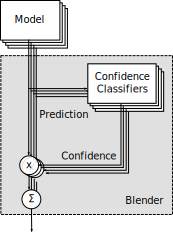
\includegraphics{gated}}
\caption{Gated Classifier Model.  Note that \emph{all} confidence classifiers receive the value of \emph{all} models, not just the one for which it is generating a confidence value.}
\label{fig:gated}
\end{center}
\vskip -0.2in
\end{figure} 

Several definitions of ``accurate'' were tried.  For the AUC task, we said that a prediction of $1 \leq \hat{x} < 3$ was accurate for the $-1$ label, and that $3 \leq \hat{x} \leq 5$ for the $+1$ class.  For RMSE, we tried to learn directly the error (difference between the label and the prediction) and a binary function of whether $|x - \hat{x}| < 1$ (whether the predicted value was within one star of the correct value).  Crucially, each confidence function had the benefit of information about the other model's predictions in order to generate its value.

It proved to be extremely difficult to learn useful gating functions.  The output of the function tended to be nearly identical over all input models, and thus the gating returned a value close to the average of the models.

\subsection{Decompositions}

By decomposition, we mean a way of reducing a set of $1151\times50000$ independent values (the outputs of all of the models over all examples) into a smaller dimensional space that preserves as much of the behaviour of the 1151 values\footnote{In this section, we use numbers from the Large task for concreteness.}.

These techniques are also known as ``information bottleneck'' methods or auto-encoders, tend to use some kind of a factorisation (explicit or implicit) to approximate a dataset with a large number of free parameters with a much smaller number of free parameters (for example, 50 or 200).
They work by learning an (encoder, decoder) pair.  The encoder reduces the 1151 dimensional input vector into a smaller internal representation.  The decoder takes the encoded vector and reproduces the 1151 values as much as possible.  A good encoder/decoder pair will do this without introducing much of an error.  Frequently, the effect of the (encode, decode) sequence will be to remove noise from the input whilst keeping its essential characteristics.  The encoded values can then be said to represent the deep structure of the data.

None of these techniques need to know the values of the ratings: they model the joint distribution of the input models.
They can be trained on an unlabelled set of data (for example, the testing set) to avoid biasing the training set.

\subsubsection{Singular Value Decomposition}

The simplest decomposition used was the SVD \cite{deerwester90}.  It uses linear algebra to generate an optimal reduced rank representation of a series of models.

Applying the SVD to a matrix $M$ breaks it down as follows:

\begin{equation}
M = U \Sigma V^T
\end{equation}

where $M$ (for the large contest) is the $50,000 \times 1151$ matrix of the model outputs, $U$ is a $50,000 \times 1151$ matrix of left-singular orthonormal vectors, $\Sigma$ is a $1151 \times 1151$ diagonal matrix with diagonal entries $[ \sigma_1 \sigma_2 \ldots \sigma_{1151}]$ and $V$ is a $1151 \times 1151$ matrix of right-singular orthonormal vectors.

The $\sigma$ values in $\Sigma$ are all non-negative and are in decreasing order of magnitude.  In order to reconstruct the best possible approximation of $M$ of rank $n$, it is sufficient to set

\begin{equation}
M \approx \hat{M} = U_n \Sigma_N V_N^T
\end{equation}

where $\hat{M}$ is a $50,000 \times 1151$ rank-$n$ approximation to $M$, $U_n$ is a $50,000 \times n$ matrix containing the first $n$ columns of $U$, $\Sigma_n$ is a $n \times n$ diagonal matrix containing the first $n$ rows and columns of $\Sigma$, and $V_n$ is a $1151 \times n$ matrix containing the first $n$ columns of $V$.  The error of any element in $M$ is bounded by the magnitude of the excluded singular values $\sum_{i=n+1}^{1151} \sigma_i$.

This matrix can be used to reduce an 1151 element model vector $\mathbf{x}$ into a $n$-dimensional representation $\mathbf{z}$ which contains as much of the information in $\mathbf{x}$ as possible.  Simply take

\begin{equation}
\label{eqn:svd-encode}
\mathbf{z} = \Sigma_n^{-1} V_n^T \mathbf{x} .
\end{equation}

The features in $\mathbf{z}$ contain as much as possible of the information in $\mathbf{x}$, but in much fewer dimensions (typical values of $n$ used in the challenge were 50, 100 and 200), and as a result have much of the noise removed.  Even if the number of dimensions is not reduced, the $\mathbf{z}$ values tend to make better features for classification as they are orthogonal from each other.

We can also produce $\hat{\mathbf{x}}$, which is a reconstituted version of $\mathbf{x}$ produced from $\mathbf{z}$:

\begin{equation}
\hat{\mathbf{x}} = V_n \Sigma_n \mathbf{z}
\end{equation}

and measure its error:

\begin{equation}
\label{eqn:decomp-error}
E = || \mathbf{x - \hat{x}} ||
\end{equation}

If $E$ is small, the information in $\mathbf{z}$ was sufficient to capture all of the information in $\mathbf{x}$.  If $E$ is large, it means that one or more of the dimensions excluded from the decomposition was important.


\subsubsection{Denoising Auto-Encoder Decomposition}

One problem with the singular value decomposition is that the the decomposition is entirely linear.  A denoising auto-encoder \cite{Vincent-TR1316} can be used to generate a non-linear decomposition, which can approximate a much larger set of (non-linear) underlying phenomena.

The goal of an auto encoder is to learn the identity function: two functions $f(\cdot)$ and $g(\cdot)$ such that $f(g(\mathbf{x})) = \mathbf{x}$.  Generally, in order to be interesting an auto-encoder will include some kind of restriction: for example, the number of dimensions in the range of $f$ is smaller than the number of dimensions in its domain.

In neural networks, the most commonly used formulation shares an activation matrix $\mathbf{W}$ between the forward and reverse directions:

\begin{equation}
\label{eqn:autoencoder-encode}
\mathbf{z} = f(\mathbf{x}) = t(W\mathbf{x} + \mathbf{b})
\end{equation}

\begin{equation}
\label{eqn:autoencoder-decode}
\hat{\mathbf{x}} = g(\mathbf{z}) = t(W^T\mathbf{z} + \mathbf{c})
\end{equation}

When $t(\cdot)$ is a non-linear squashing function such as $t(\mathbf{x}) = \tanh(\mathbf{x})$, we can use back-propagation to learn a nonlinear decomposition.

Note that these auto-encoders can be stacked one on top of the other, so that we apply all of the forward functions one after the other and then all of the reverse directions in the opposite order.

In order to make the auto encoder generalise (and learn higher level features), we need to either a) add noise to the input (and train the auto encoder to remove the noise) and/or b) create an ``information bottleneck'', by reducing the number of neural network units lower down in the stack.  This leads to the architecture used in the challenge, which is shown in figure \ref{fig:autoencoder-decomposition}:

\begin{figure}[ht]
\vskip 0.2in
\begin{center}
\centerline{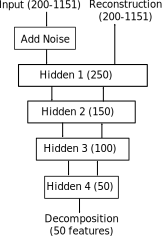
\includegraphics{auto-encoder}}
\caption{Denoising auto-encoder decomposition used in the challenge.}
\label{fig:autoencoder-decomposition}
\end{center}
\vskip -0.2in
\end{figure} 

In order to train the auto-encoders, a standard back-propagation algorithm can be used to perform gradient descent on the parameter space.  Normally, a stack of auto encoders will be trained a layer at a time on the output of the previous layer (in a greedy manner), although it is possible to train the entire stack at once.  Both methods were used in the challenge.

\paragraph{Improvements}

Several improvements were made to the auto-encoder model described previously.

Firstly, it is known that a linear neural network under the right conditions will approximate the singular value decomposition.  It would make sense for the auto encoder described in the previous section to be able to do so.  However, if we set $t$ to the identity function and $W = \Sigma_n^{-1} V_n^T$ in \ref{eqn:autoencoder-encode} as in equation \ref{eqn:svd-encode} (ignoring the bias terms), we get

\begin{equation}
\mathbf{z} = \Sigma_n^{-1} V_n^T \mathbf{x}
\end{equation}

and so

\begin{equation}
\hat{\mathbf{x}} = V_n \left( \Sigma_n^{-1} \right)^T \Sigma_n^{-1} V_n^T \mathbf{x} = \Sigma_n^{-2} \mathbf{x}
\end{equation}

where we rely on the fact that $V^T V = I$ due to $V$ being orthonormal.

Thus, this auto-encoder can only reproduce its input, no matter the dimensionality, if all of the singular values of our data matrix are unitary, which is rarely true.  The alternative of not including $\Sigma_n$ in the encoder function is not satisfactory as this will cause the neurons corresponding to the high-valued singular values to dominate the training.

To rectify this problem, we added two extra terms to the decoding function \ref{eqn:autoencoder-decode}:

\begin{equation}
\label{eqn:autoencoder-decode-improved}
\hat{\mathbf{x}} = t(D \mathbf{W}^T E \mathbf{z} + \mathbf{c})
\end{equation}

where $D$ and $E$ are diagonal matrices that control the input and output gain of the activation matrix $W^T$.  Then, by setting $W = \Sigma_n^{-1} V_n^T$, $E = I$ and $D = \Sigma_n^{-2}$ we can achieve our goal of emulating the SVD.

A second improvement was made to the treatment of noisy inputs.  In \cite{Vincent-TR1316}, noisy inputs are simply set to zero.  This causes problems with the auto encoder, as the same weight in $W$ is simultaneously trying to reject noise, contribute to the hidden state and reproduce the output from the hidden state.  Instead, as plenty of data was available, we used a separate activation matrix $W_N$ for the noisy inputs.  Those inputs which were chosen to be noisy were assumed to have an input value of 1 and connected via $W_N$ instead of $W$ to the hidden layer.  This change significantly increased the accuracy of the reconstruction in the no-noise case\footnote{It has not been proved that an auto-encoder needs to do a good job of reconstruction in order to provide a useful decomposition, but intuitively it seems necessary.}.

The third improvement was made in the addition of noise.  It was observed that the auto-encoders actually were better at reproducing the (noiseless) input when that input had noise added than when it was presented in a pristine state.
This was because the auto-encoders were depending upon a certain number of their inputs having the value zero: if 20\% noise is added and an internal state represents the mean of the inputs, then that state is going to be 125\% the mean when no noise is present.
In order to prevent the auto-encoders from expecting the noise to be present, every second example was presented with no noise added.  Again, this change significantly increased the auto-encoder's reconstruction performance in the noiseless case.

\subsection{Derived Features}

In order to make it easier for the classifiers to work, the component models were augmented with several derived features:

\begin{itemize}
\item The minimum, maximum, mean and standard deviation of the model outputs;
\item For of the 10 highest ranking models:
  \begin{itemize}
    \item The minimum, maximum and mean value;
    \item Variables comparing the spread of values over these 10 models and the spread of values over all of the models;
    \item For each of the 10 models, the output of the model and the number of standard deviations from the mean of all models;
    \item The difference between the output of this model and the closest integer;
    \item If a decomposition was used, the error of the reconstruction of this model by the decomposition;
  \end{itemize}
\item The output of the decomposition (SVD or Denoising Auto-Encoder), if there was any;
\item The RMS error of the decomposition, as in equation \ref{eqn:decomp-error}.

\end{itemize}

\subsection{Multiple Models}

Highly non-linear algorithms such as decision trees, regression trees and especially meta-algorithms like Adaboost tend to have big problems dealing with noise.
One way of mitigating this effect is by averaging models trained over random subsets of the data.  The following techniques were used:

\begin{itemize}
\item Random decision trees and regression trees were used to train the final classifier in the gated models.  The most successful model used 500 bags (with random selection of examples) of 10 iterations of boosted random decision trees (with a random subset of the features).
\item Wherever regression (linear or logistic) was used, the regression was performed multiple (20-500) times and the average of the models taken.  A random subset of examples and of features was chosen.
\end{itemize}

\subsection{Ridge Regression}

Ridge regression was used in place of linear regression in all circumstances, including within the Iteratively Reweighed Least Squares routines used to calculate the logistic regression coefficients \cite{komarek2005}.

Ridge regression is a regularised form of linear regression, that penalises high weights in the model coefficients $\mathbf{x}$.  The algorithm calculates the value of the vector $\mathbf{x}$ that minimises the following error:

\begin{equation}
  E = ||W\mathbf{x} - \mathbf{b}|| + \lambda ||\mathbf{b}||^2 \leftarrow \mbox{Regularisation term}
\end{equation}

The coefficient $\lambda$ describes the trade-off between fitting the data and reducing the size of the parameters in $\mathbf{x}$.  The optimal value of $\lambda$ can be efficiently calculated using leave-one-out cross validation.

Ridge regression also has the advantage of working well on rank-deficient or poorly conditioned problems, unlike standard linear regression.  
This is important in the context of this work: there are a lot of small, but not insignificant singular values in the data. 

\subsection{Deep Neural Network Model}

The denoising auto-encoders are trained with no knowledge of the target feature.
By adding an extra output layer or two and training the entire resulting network with back-propagation, the features that it has learnt in its internal representation can be fine-tuned to help produce a target output (here, the label for the AUC or RMSE model).  Figure \ref{figure:deepnet} illustrates the architecture.

\begin{figure}[t]
\vskip 0.2in
\begin{center}
\centerline{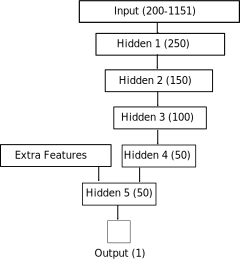
\includegraphics{deepnet}}
\caption{Deep Network Model.}
\label{figure:deepnet}
\end{center}
\vskip -0.2in
\end{figure} 

\section{Method}

In order to generate results, a large number of predictors were trained implementing the ideas described above.  Each of these predictors was trained on 80\% of the training data, with the other 20\% (always the same part) held out in order to train the final blending model.  When each predictor was run, it created:
%
\begin{enumerate}
\item A blending results file containing the model's unbiased prediction for each entry of the 20\% of final blending data held out;
\item A submission results file containing the model's prediction for each entry of the scoring set (for which labels weren't available).
\end{enumerate}
%
Once all of the files were available, they were combined using a final blending stage, the result of which was the submitted result.

\subsection{Decompositions}
\label{sec:decompositions}

A total of four decompositions were generated: one SVD decomposition and three denoising auto-encoder decompositions.  Table \ref{table:dnae-decompositions} shows the parameters used.  In each case, the layer sizes are as indicated in \ref{fig:autoencoder-decomposition}.  Learning rates were set via manual tuning.  On the small dataset, 80\% of the examples were randomly selected on each iteration; 50\% on the medium and 10\% on the large.  The presentation order of examples was random.  The bug referred to in the table when training DNAE1 was the use of the non-noisy input vector when back-propagating, leading to noisy inputs being incorrectly updated.

\begin{table}
\caption{Denoising Auto-Encoder Decompositions.  Layer Iter is the number of back-propagation iterations that each layer was trained by itself, Stack Iter is the number of back-propagation iterations that the entire stack was trained after each layer was added.  Bug indicates the presence of a bug described in section \ref{sec:decompositions}.}
\label{table:dnae-decompositions}
\vskip 0.15in
\begin{center}
\begin{small}
\begin{sc}
\begin{tabular}{lrrr}
\hline
\abovespace\belowspace
Model & Layer Iter & Stack Iter & Bug \\
\hline
\abovespace
dnae1 & 500    & 500 & $\surd$ \\
dnae2 & 800    &   0 &         \\
\belowspace
dnae3 & 400    & 200 &         \\
\hline
\end{tabular}
\end{sc}
\end{small}
\end{center}
\vskip -0.1in
\end{table}


\subsection{Multiple Regression}

The multiple regression predictors turned out to be the most powerful, particularly in the RMSE task.  This is largely due to their ability to reject noise due to their inherent smoothness, the regularisation provided by ridge regression and the smoothing provided by the random selection of features and examples.

Table \ref{table:multiple-regression-models} describes the parameters for the different models.  In all cases, 500 separate regression models were combined (linear regression for the RMSE task; logistic regression for the AUC task) on 6,000 randomly selected examples.  On the small task, the number of features sampled and the decomposition order were set to 100; for the medium task 150 and for the large task 200.  When extra features were used, they were sampled along with the model outputs.

\begin{table}
\caption{Multiple Regression Models Used}
\label{table:multiple-regression-models}
\vskip 0.15in
\begin{center}
\begin{small}
\begin{sc}
\begin{tabular}{llc}
\hline
\abovespace\belowspace
Model & Decomposition & Extra Features \\
\hline
\abovespace
mr1   &        &         \\
mr2   & SVD    &         \\
mr3   & SVD    & $\surd$ \\
mr4   & DNAE1  &         \\
mr5   & DNAE1  & $\surd$ \\
mr6   & DNAE2  &         \\
mr7   & DNAE2  & $\surd$ \\
mr8   & DNAE3  &         \\
\belowspace
mr9   & DNAE3  & $\surd$ \\
\hline
\end{tabular}
\end{sc}
\end{small}
\end{center}
\vskip -0.1in
\end{table}


\subsection{Deep Neural Networks}

Table \ref{table:deep-net-models} describes the deep network models used.  Each of these had an architecture with 250, 150, 100 and 50 units (from the denoising auto-encoders) and another 50 hidden units feeding into the single unit output layer.  The extra features are not fed in the top, but directly into the 50 unit hidden layer, bypassing the auto-encoder.  Standard $tanh$ units were used.

\begin{table}
\caption{Deep Network Models Used}
\label{table:deep-net-models}
\vskip 0.15in
\begin{center}
\begin{small}
\begin{sc}
\begin{tabular}{llc}
\hline
\abovespace\belowspace
Model & Decomposition & Extra Features \\
\hline
\abovespace
dn1   & DNAE2  & $\surd$  \\
dn2   & DNAE2  &   \\
dn3   & DNAE3  &   \\
\belowspace
dn4   & DNAE3  & $\surd$  \\
\hline
\end{tabular}
\end{sc}
\end{small}
\end{center}
\vskip -0.1in
\end{table}


\subsection{Gated Merger}

Several models of the ``gated'' merger described in \ref{sec:state-space-accuracy} were tried.  This model tended to perform reasonably well for the AUC task, but poorly for the RMSE task.  Presumably, this is because the two-stage nature of the model caused the noise to be amplified between the stages.

The models differed in which decomposition they used (no decomposition, the SVD or the denoising auto-encoders), whether or not they used extra features, and the technique used for the final score once the confidence-modified values had been produced.  Table \ref{table:gated-models} shows these parameters.


\begin{table}
\caption{Gated Merger Models Used}
\label{table:gated-models}
\vskip 0.15in
\begin{center}
\begin{small}
\begin{sc}
\begin{tabular}{lccc}
\hline
\abovespace\belowspace
Model & Decomp. & Blend RMSE & Blend AUC \\
\hline
\abovespace
gated   & SVD(200)  & LR & Rand Forest  \\
gated2  &           & LR & Rand Forest  \\
gated3  & DNAE1     & LR & Rand Forest  \\
gated4  & DNAE2     & LR & Rand Forest  \\
gated5  & DNAE3     & LR & Rand Forest  \\
gated6  & DNAE3     & Rand Forest & N/A  \\
\belowspace
gated7  & DNAE3     & Multi LR & N/A   \\
\hline
\end{tabular}
\end{sc}
\end{small}
\end{center}
\vskip -0.1in
\end{table}

\subsection{Classifier Models}

For the RMSE data, two classifier models were used.  One, \texttt{rtrees} used a random forest of 200 regression trees.  The other, \texttt{mclass}, learnt a binary classifier for several discrete movie ratings (1, 2, 3, 4 or 5 stars; 2-5 stars; 3-5 stars; 4-5 stars) using a random forest of 5000 decision trees, and combined these predictions using linear regression.  Neither model performed particularly well.

\subsection{Final Blending}

Final blending was performed using a cross-validation training on the 20\% held out data.  The held out data was broken into 10 folds, and 10 different multiple regression blenders were trained, each training on 9 and leaving out one fold.
The performance of the merged model on the entire 20\% held out was then evaluated.
The challenge submission files were generated by running the 10 multiple regression blenders over the entire testing set, and averaging the results.

This strategy was adapted in order to reduce the impact that a ``rogue'' model (with a high error rate, or over-fit on its training data) would have on the final blend.  It is unlikely that performing (yet another) round of blending of already blended models would significantly improve the results; this bootstrapping with no additional leverage.  Uniform linear blending appeared to work just as well.

\subsection{Implementation}

In practise, this challenge turned out to be as much about software engineering as about data mining.

The biggest reason for this was the amount of noise in the data.  This necessitated that models be run many times (up to 500) and the results averaged, with a corresponding increase in compute time.

Due to the limited hardware resources available\footnote{One quad core ``hyper-threaded'' (8 virtual cores) desktop machine with 6GB of RAM, one dual core laptop with 2GB of RAM} and the large number of tasks, it was necessary that the software be both memory and CPU efficient.
The entire code was vectorised to take advantage of the vector unit, multi-threaded\footnote{On the desktop machine, 8 threads were run to fully exploit the hyper-threaded processor} and the bottlenecks were profiled and carefully optimised.  Single precision arithmetic was used wherever possible\footnote{It is frequently not possible.  For example, whenever accumulating a series of numbers it is necessary to accumulate in double precision even if the numbers being accumulated are only in single precision.} due to its two-fold advantage in execution speed on modern hardware.

To save memory bandwidth, parameters were stored using as small a precision as possible and care was taken not to duplicate memory when splitting datasets into training and validation sets.

The fact that there were six different tasks (AUC and RMSE for the small, medium and large datasets) also increased the amount of CPU time and engineering work required, especially in manually tuning the back-propagation parameters.

In the end, about 5,000 lines of C++ code were written for the challenge directly, and about 10,000 lines added to the underlying machine learning library (primarily the code to perform Ridge Regression and the denoising auto-encoder routines).  The entire set of results could be reproduced in about 24 hours on a consumer desktop PC.

The software was developed on Linux.  The only significant external libraries used were LAPACK and BLAS for the linear algebra routines.

\subsection{Open Source}

The source code for this submission is available.  The machine learning library used to perform the heavy lifting is available at http://bitbucket.org/jeremy\_barnes/jml/.  The source code of the actual AUSDM submission is available at http://github.com/jeremybarnes/ausdm.  Both are available under the Affero GNU Public License version 3.  The \texttt{ausdm} repository also contains some of the data files used in the building of the results.

\section{Results}

\subsection{Diversity and Independence of Model Predictions}
\label{sec:svd-decomposition-results}

Table \ref{table:sv-distributions} shows the distribution of singular values over the six tasks.  The top part lists values of the singular values; the bottom part lists counts of various categories.

The spread of the singular values give an idea of the diversity of the models in the data: the small singular values correspond to models that don't contain much more information over and above those with higher singular values.  The small task appears to have little redundancy in the provided models, whereas the large task has significant redundancy, and potentially even models that were (pre-blended) linear combinations of others.

% cat ../loadbuild/gated/L_rmse_official.txt.log | grep singular_values | sed 's/singular_values = { //g;s/}//g' | tr ' ' '\n' | awk 'BEGIN { min=10000.5; lessone = 0;  less01 = 0;  } { if ($1 > max) max = $1;  if ($1 < min) min = $1; if ($1 > 100) ++hundred;  if ($1 > 10) ++ten;  if ($1 > 1) ++one;  if ($1 > 0.1) ++pointone; } END { print max, hundred, ten, one, pointone; }'

\begin{table}[t]
\caption{Independence and Conditioning of Models.  The singular values of each data matrix were taken.  The top half lists values (highest, second highest and lowest); the bottom half shows a histogram over orders of magnitude.}
\label{table:sv-distributions}
\vskip 0.15in
\begin{center}
\begin{small}
\begin{sc}
\begin{tabular}{lrrrrrr}
\hline
\abovespace\belowspace
& \multicolumn{2}{c}{Small} & \multicolumn{2}{c}{Medium} & \multicolumn{2}{c}{Large} \\
Type & AUC & RMS & AUC & RMS & AUC & RMS \\
\hline
\abovespace
Top        & 936 & 806 & 674 & 1040 & 2830   & 3538 \\
2nd        &  69 &  55 &  83 &   77 &  257   &  253 \\
min        & 0.9 & 0.9 & 0.4 &  0.8 & $10^{-5}$& $10^{-5}$ \\
\abovespace
$> 100$    &   1 &   1 &   1 &    1 &    9   &    9 \\
$> 10$     &  72 &  59 &  88 &   87 &  433   &  428 \\
$> 1$      & 199 & 197 & 247 &  249 & 1071   & 1074 \\
$> 0.1$    & 200 & 200 & 250 &  250 & 1143   & 1143 \\
\belowspace
$\leq 0.1$ &   0 &   0 &   0 &    0 &    8   &    8 \\
%n          & 200 & 200 & 250 &  250 & 1151   & 1151 \\
\hline
\end{tabular}
\end{sc}
\end{small}
\end{center}
\vskip -0.1in
\end{table}

\subsection{Decompositions}

Table \ref{table:dnae-decomposition-accuracy} shows the reconstruction accuracy of the decompositions of different orders over the training sets.
The reconstruction accuracy increases as we move from DNAE1 to DNAE2 to DNAE3, but that they aren't as efficient at reproducing the data as the SVD.
This is a disappointing result: the non-linearities were either not being exploited or were not useful.
DNAE3 is particularly interesting, as it shows the effect of training the stack as a whole rather than each layer individually.  Doing so reduces the efficiency of the individual layers as separate auto-encoders, but to improves the entire stack.

\begin{table}[t]
\caption{Decomposition reconstruction accuracies.  These are the total RMSE over all inputs for different decompositions as the order (dimensionality) of the decomposition varies.}
\label{table:dnae-decomposition-accuracy}
\vskip 0.15in
\begin{center}
\begin{small}
\begin{sc}
\begin{tabular}{crrrrr}
\hline
\abovespace\belowspace
Set & Order & SVD & DAE1 & DAE2 & DAE3 \\
\hline
\abovespace
     & 250 & 0.00 & 0.86 & 0.81 & 6.51 \\
S    & 150 & 0.20 & 1.48 & 1.15 & 3.51 \\
AUC  & 100 & 0.44 & 1.99 & 1.30 & 1.92 \\
     &  50 & 0.72 & 2.22 & 1.40 & 0.92 \\
\abovespace
     & 250 & 0.00 & 0.62 & 0.62 & 3.58 \\
M    & 150 & 0.30 & 1.09 & 1.02 & 3.44 \\
AUC  & 100 & 0.48 & 1.52 & 1.42 & 2.87 \\
     &  50 & 0.74 & 1.97 & 1.80 & 0.90 \\
\abovespace
     & 250 & 1.00 & 2.08 & 2.18 & 17 \\
L    & 150 & 1.31 & 3.24 & 3.05 & 4.88 \\
AUC  & 100 & 1.52 & 4.18 & 3.74 & 2.98 \\
     &  50 & 1.84 & 5.01 & 4.34 & 2.08 \\
\abovespace
     & 250 & 0.99 & 2.31 & 2.51 & 23 \\
L    & 150 & 1.30 & 3.58 & 3.42 & 5.52 \\
RMSE & 100 & 1.51 & 4.56 & 4.08 & 2.84 \\
\belowspace
     &  50 & 1.82 & 5.38 & 4.49 & 2.08 \\
\hline
\end{tabular}
\end{sc}
\end{small}
\end{center}
\vskip -0.1in
\end{table}

Looking at the results of the \texttt{gated} (SVD decomposition), \texttt{gated3} (DNAE1 decomposition), \texttt{gated4} (DNAE2 decomposition) and \texttt{gated4} (DNAE3 decomposition) algorithms (which differ only in the decomposition used), it appears that the SVD decomposition is the most useful, followed by the DNAE3, DNAE2 and DNAE1 decompositions.  These results are disappointing.  It is possible that allowing interactions between the features (as in \cite{larochelle2009}) would improve matters, but as they stand these results would have to be considered a failure.

\subsection{AUC Results}

We present the AUC results in table \ref{table:auc-results}, showing the performance of both the component models and the blended result.  The table for each task contains two columns of numerical information.  The first describes the error score of the model, with the lift (reduction in error) as compared with the baseline model, multiplied by 1000.  The second shows the average blending weight of the model (over 10 folds) as well as the standard deviation in this value.  The blending weights give an idea of the importance of the model to the final result.

%(cat ../loadbuild/merged/S_auc_official.txt.log; echo "next"; cat ../loadbuild/merged/M_auc_official.txt.log; echo "next"; cat ../loadbuild/merged/L_auc_official.txt.log; echo "next") | awk -v baseline1=0.0597 -v baseline2=0.3384 -v baseline3=0.1635 -f tabulate_results.awk | sort

\begin{table*}[t]
\caption{AUC Blending Results.  The lift is 1000 times the improvement over the baseline score.  The weight values, which describe the blending weight in the final model, are reported as mean $\pm$ standard deviation.}
\label{table:auc-results}
\vskip 0.15in
\begin{center}
\begin{small}
\begin{sc}
\begin{tabular}{l|rr r|rr r|rr r}
\hline
\abovespace\belowspace
Task & \multicolumn{3}{|c}{Small} & \multicolumn{3}{|c}{Medium} & \multicolumn{3}{|c}{Large} \\
Model
& AOC & Lift & Weight 
& AOC & Lift & Weight 
& AOC & Lift & Weight \\
\hline
\abovespace
dn1        & 0.0585 &   1.2 & -0.36$\pm$0.32& 0.3299 &   8.5 &  0.04$\pm$0.23& 0.1581 &   5.4 & -0.41$\pm$0.20 \\ 
dn2        & 0.0611 &  -1.4 &  0.20$\pm$0.19& 0.3431 &  -4.7 & -0.51$\pm$0.22& 0.1634 &   0.1 & -0.05$\pm$0.21 \\ 
dn3        & 0.0611 &  -1.4 &  0.19$\pm$0.17& 0.3432 &  -4.8 & -0.49$\pm$0.19& 0.1634 &   0.1 & -0.60$\pm$0.23 \\ 
dn4        & 0.0585 &   1.2 & -0.34$\pm$0.30& 0.3300 &   8.4 &  0.05$\pm$0.24& 0.1581 &   5.4 & -0.83$\pm$0.31 \\ 
\abovespace
gated      & 0.0565 &   3.2 &  0.80$\pm$0.23& 0.3239 &  14.5 &  0.60$\pm$0.25& 0.1497 &  13.8 &  1.09$\pm$0.27 \\ 
gated2     & 0.0584 &   1.3 &  0.26$\pm$0.24& 0.3318 &   6.6 & -0.08$\pm$0.27& 0.1528 &  10.7 &  0.32$\pm$0.24 \\ 
gated3     & 0.0592 &   0.5 & -0.55$\pm$0.35& 0.3282 &  10.2 &  0.09$\pm$0.29& 0.1524 &  11.1 &  0.19$\pm$0.32 \\ 
gated4     & 0.0586 &   1.1 & -0.02$\pm$0.29& 0.3303 &   8.1 & -0.26$\pm$0.44& 0.1528 &  10.7 & -0.64$\pm$0.33 \\ 
gated5     & 0.0580 &   1.7 &  0.37$\pm$0.14& 0.3264 &  12.0 &  0.11$\pm$0.31& 0.1519 &  11.6 &  0.32$\pm$0.13 \\ 
\abovespace
mr1        & 0.0639 &  -4.2 &  0.23$\pm$0.33& 0.3208 &  17.6 &  0.47$\pm$0.47& 0.1581 &   5.4 & -0.08$\pm$0.39 \\ 
mr2        & 0.0633 &  -3.6 &  0.18$\pm$0.33& 0.3203 &  18.1 &  0.46$\pm$0.49& 0.1584 &   5.1 & -0.88$\pm$0.30 \\ 
mr3        & 0.0575 &   2.2 &  0.57$\pm$0.51& 0.3174 &  21.0 &  0.03$\pm$0.51& 0.1499 &  13.6 &  1.84$\pm$0.69 \\ 
mr4        & 0.0573 &   2.4 &  0.39$\pm$0.27& 0.3196 &  18.8 &  0.82$\pm$0.34& 0.1508 &  12.7 & -0.75$\pm$0.38 \\ 
mr5        & 0.0574 &   2.3 & -0.29$\pm$0.29& 0.3128 &  25.6 &  0.80$\pm$0.44& 0.1485 &  15.0 &  1.58$\pm$0.47 \\ 
mr6        & 0.0573 &   2.4 &  0.51$\pm$0.30& 0.3201 &  18.3 &  0.61$\pm$0.22& 0.1505 &  13.0 &  0.13$\pm$0.29 \\ 
mr7        & 0.0573 &   2.4 & -0.21$\pm$0.25& 0.3135 &  24.9 &  0.65$\pm$0.42& 0.1485 &  15.0 &  0.74$\pm$0.43 \\ 
mr8        & 0.0572 &   2.5 &  0.90$\pm$0.60& 0.3186 &  19.8 & -0.06$\pm$0.30& 0.1500 &  13.5 &  2.04$\pm$0.57 \\ 
mr9        & 0.0574 &   2.3 & -0.04$\pm$0.16& 0.3146 &  23.8 &  0.24$\pm$0.24& 0.1484 &  15.1 &  0.58$\pm$0.66 \\ 
%\abovespace
%bias       &        &       & -1.09$\pm$0.46&        &       & -2.10$\pm$0.34&        &       & -2.57$\pm$0.32 \\ 
\abovespace\belowspace
combined   & 0.0571 &   2.6 &  & 0.3144 &  24.0 &  & 0.1461 &  17.4 &   \\ 
\hline
\end{tabular}
\end{sc}
\end{small}
\end{center}
\vskip -0.1in
\end{table*}

The multiple regression models appear to be the most consistently accurate, followed by the gated models.  The deep network models appeared to be used mostly to attenuate noise, as their blending weights were more negative than positive.  The greatest lift was obtained on the medium task (which was also the hardest, and consequently had the most scope for improvement).  A significant improvement was also obtained on the large task.  The lift on the small task was small, but (as will be discussed below) there was not much scope for improvement due to the noise ceiling.

It is instructive to compare the multiple regression models to determine the effect of the various strategies.  Recall from table \ref{table:multiple-regression-models} that \texttt{mr1} contained only the component models, \texttt{mr2} augmented this with an SVD and \texttt{mr3} with the extra features.  Any improvement in \texttt{mr1} is therefore attributable to the calibration of the component scores from the RMSE (quadratic error) task to the AUC (linear error) task.

It seems that most of the improvement is due to the extra features, as \texttt{mr1} and \texttt{mr2} are not significantly different, but \texttt{mr3} is always significantly better than the others.  On the other hand, it appears from the rest of the \texttt{mr} results that, especially on the large task, the DNAE models provide a useful substitute for the extra features, whereas the SVD does not.  Or in other words, the DNAE decompositions manage to implicitly capture most of the information in the extra features whereas the SVD does not.

The deep network models (\texttt{dn1} to \texttt{dn4}) did not perform well, but were improved by adding the extra features.

In all cases, the \texttt{gated} model worked better than \texttt{gated2} through \texttt{gated4}.  As these models always had extra features available, this shows that the SVD decomposition is more useful than the DNAE decompositions.

Overall, the AUC results successfully provided a modest lift.  It was particularly encouraging to see that the merged model on the large dataset was significantly more accurate than any of its component predictors.

\subsubsection{Noise}

The small AUC task was particularly noisy, and only a small improvement seems possible.
One explanation for this would be the selection of target values for this task, which are $(-1 \rightarrow 1)$ and $(+1 \rightarrow 5)$.  
These two values, and particularly the value 1, are associated with extreme emotional reactions to films by users, much of which cannot realistically be modelled\footnote{How is a computer to know that this was the favourite film of a hated ex and is thus terrible by association?}.
The relative scarcity of 1 rankings in the dataset also makes them more susceptible to noise (accidental mouse clicks, distraction, cats walking on keyboards, etc), which are probably uniformly distributed over the dataset.
When adapting to the large and particularly the medium task at the end of the challenge, it was observed that noise was much less of a problem.

\subsection{RMSE Results}

%cat ../loadbuild/merged/S_rmse_official.txt.log; echo "next"; cat ../loadbuild/merged/M_rmse_official.txt.log; echo "next"; cat ../loadbuild/merged/L_rmse_official.txt.log; echo "next") | awk -v baseline1=0.4398 -v baseline2=0.4307 -v baseline3=0.4419 -f tabulate_results.awk | sort

\begin{table*}[t]
\caption{RMSE Blending Results.  The lift is 1000 times the improvement over the baseline score.  The weight values, which describe the blending weight in the final model, are reported as mean $\pm$ standard deviation.}
\label{table:rmse-results}
\vskip 0.15in
\begin{center}
\begin{small}
\begin{sc}
\begin{tabular}{l|rr r|rr r|rr r}
\hline
\abovespace\belowspace
Task & \multicolumn{3}{|c}{Small} & \multicolumn{3}{|c}{Medium} & \multicolumn{3}{|c}{Large} \\
Model
& RMSE & Lift & Weight 
& RMSE & Lift & Weight 
& RMSE & Lift & Weight \\
\hline
\abovespace
dn1        & 0.4422 &  -2.4 &  0.02$\pm$0.01& 0.4332 &  -2.5 &  0.04$\pm$0.02& 0.4442 &  -2.3 & -0.06$\pm$0.03 \\ 
dn2        & 0.4485 &  -8.7 &  0.02$\pm$0.03& 0.4407 & -10.0 &  0.03$\pm$0.02& 0.4495 &  -7.6 & -0.02$\pm$0.04 \\ 
dn3        & 0.4486 &  -8.8 &  0.02$\pm$0.04& 0.4409 & -10.2 &  0.03$\pm$0.03& 0.4497 &  -7.8 &  0.02$\pm$0.07 \\ 
dn4        & 0.4421 &  -2.3 &  0.02$\pm$0.01& 0.4332 &  -2.5 &  0.03$\pm$0.02& 0.4442 &  -2.3 & -0.06$\pm$0.04 \\ 
\abovespace
gated      & 0.4500 & -10.2 &  0.07$\pm$0.04& 0.4462 & -15.5 &  0.02$\pm$0.04& 0.4418 &   0.1 &  0.09$\pm$0.04 \\ 
gated2     & 0.4409 &  -1.1 &  0.08$\pm$0.04& 0.4315 &  -0.8 &  0.07$\pm$0.04& 0.4414 &   0.5 &  0.09$\pm$0.04 \\ 
gated3     & 0.4554 & -15.6 & -0.04$\pm$0.03& 0.4420 & -11.3 &  0.02$\pm$0.04& 0.4428 &  -0.9 &  0.05$\pm$0.04 \\ 
gated4     & 0.4490 &  -9.2 &  0.03$\pm$0.03& 0.4393 &  -8.6 &  0.00$\pm$0.03& 0.4419 &   0.0 &  0.04$\pm$0.05 \\ 
gated5     & 0.4620 & -22.2 &  0.03$\pm$0.03& 0.4487 & -18.0 & -0.04$\pm$0.04& 0.4460 &  -4.1 &  0.01$\pm$0.02 \\ 
gated6     & 0.4421 &  -2.3 &  0.03$\pm$0.04& 0.4317 &  -1.0 &  0.03$\pm$0.04& 0.4421 &  -0.2 &  0.02$\pm$0.05 \\ 
gated7     & 0.4394 &   0.4 &  0.04$\pm$0.02& 0.4295 &   1.2 &  0.04$\pm$0.03& 0.4405 &   1.4 & -0.05$\pm$0.10 \\ 
\abovespace
mr1        & 0.4379 &   1.9 &  0.07$\pm$0.02& 0.4277 &   3.0 &  0.10$\pm$0.02& 0.4386 &   3.3 &  0.13$\pm$0.04 \\ 
mr2        & 0.4377 &   2.1 &  0.08$\pm$0.01& 0.4275 &   3.2 &  0.10$\pm$0.04& 0.4387 &   3.2 &  0.10$\pm$0.02 \\ 
mr3        & 0.4377 &   2.1 &  0.07$\pm$0.02& 0.4276 &   3.1 &  0.09$\pm$0.03& 0.4386 &   3.3 &  0.11$\pm$0.03 \\ 
mr4        & 0.4382 &   1.6 &  0.06$\pm$0.03& 0.4278 &   2.9 &  0.08$\pm$0.03& 0.4386 &   3.3 &  0.10$\pm$0.06 \\ 
mr5        & 0.4379 &   1.9 &  0.06$\pm$0.02& 0.4277 &   3.0 &  0.08$\pm$0.04& 0.4386 &   3.3 &  0.10$\pm$0.06 \\ 
mr6        & 0.4379 &   1.9 &  0.07$\pm$0.02& 0.4277 &   3.0 &  0.09$\pm$0.03& 0.4386 &   3.3 &  0.11$\pm$0.02 \\ 
mr7        & 0.4377 &   2.1 &  0.07$\pm$0.02& 0.4278 &   2.9 &  0.06$\pm$0.04& 0.4385 &   3.4 &  0.15$\pm$0.09 \\ 
mr8        & 0.4377 &   2.1 &  0.07$\pm$0.02& 0.4275 &   3.2 &  0.10$\pm$0.04& 0.4389 &   3.0 &  0.07$\pm$0.02 \\ 
mr9        & 0.4379 &   1.9 &  0.06$\pm$0.01& 0.4278 &   2.9 &  0.05$\pm$0.05& 0.4389 &   3.0 &  0.05$\pm$0.03 \\ 
\abovespace
mclass     & 0.4398 &   0.0 &  0.06$\pm$0.05& 0.4319 &  -1.2 &  0.02$\pm$0.03& 0.4417 &   0.2 & -0.00$\pm$0.04 \\ 
rtrees     & 0.4411 &  -1.3 &  0.05$\pm$0.05& 0.4321 &  -1.4 &  0.02$\pm$0.04& 0.4427 &  -0.8 & -0.05$\pm$0.05 \\ 
%\abovespace
%bias       &        &       &  0.00$\pm$0.02&        &       & -0.02$\pm$0.01&        &       & -0.00$\pm$0.01 \\ 
\abovespace\belowspace
combined   & 0.4381 &   1.7 &  & 0.4277 &   3.0 &  & 0.4385 &   3.4 &   \\ 
\hline
\end{tabular}
\end{sc}
\end{small}
\end{center}
\vskip -0.1in
\end{table*}

The RMSE task results presented in table \ref{table:rmse-results} are not encouraging.  The deep network results were all very poor and the gated results only rarely beat the baseline.  The multiple regression results were nearly uniform which means that the effect of the extra features and the decompositions was minimal.  The final lift obtained is far too small to be detectable by a user of such a system.  The inescapable conclusion is that we failed to achieve a significant improvement in the RMSE task.

Unlike the AUC task, final blending was ineffectual on the RMSE task: the score of the blended result was slightly worse than the best individual result\footnote{The submitted results were still the blended ones, however, as they should be more resistant to the selection bias in the validation set}.  This is probably due to there not being enough diversity in the models blended: there were only a few really distinct models with reasonable performance, and these frequently used the same features (from the DNAE, the SVD and the derived features).

\subsubsection{Criticism of quadratic metrics on noisy data}

This phenomena is probably explained by the use of a RMSE metric, and the amount of noise in the data.  The RMSE metric penalises very heavily incorrect predictions at the extreme ends of the scale: a prediction of 1 has 4 times the potential MSE error (16 points) than a prediction of 3 (4 points).  As the noise in the data increases, it becomes more and more costly to deviate significantly from the 3 prediction.

Assuming that random noise is added equally to each label, label 1 already becomes difficult to predict.  If we also consider that label 1 would most likely be used by people for emotional reactions to films (likely, some proportion of the 1 ratings are due to vitriol), they become even more difficult to model.

\paragraph{Row Breakdown}
It is instructive to break the dataset into different types of rows, based upon the ease with which a prediction can be made:
\begin{itemize}
\item \emph{easy}: all models are within one star of the correct answer;
\item \emph{possible}: at least one model is within one star of the correct answer;
\item \emph{impossible}: no model is within one star of the correct answer\footnote{It is could happen that the impossible values be clustered on both sides of the correct answer and that their mean be a good predictor, but this was not observed in the data.}.
\end{itemize}

Table \ref{table:row-types-rmse} shows the result of this breakdown on the large RMSE dataset, and the contribution of the different row types to the total MSE for the baseline model.  Considering that it is very unlikely that any improvement could be made on these positions, it is still very important to pick a good middle value for them, as they account for $1/3$ of the error. 

\begin{table}[t]
\caption{Large RMSE training set broken down by row difficulty.  In the last column, we see that 1/3 of the MSE comes from the impossible positions, which account for just 5.7\% of the data.}
\label{table:row-types-rmse}
\vskip 0.15in
\begin{center}
\begin{small}
\begin{sc}
\begin{tabular}{lrrr}
\hline
\abovespace\belowspace
Category & Freq & Avg MSE & Total MSE \\
\hline
\abovespace
Easy          & 0.329 & 0.019 & 0.0063 \\
Possible      & 0.614 & 0.198 & 0.1216 \\
Impossible    & 0.057 & 1.189 & 0.0678 \\
\abovespace\belowspace
Total         & 1.000 & 0.195 & 0.1953 \\
\hline
\end{tabular}
\end{sc}
\end{small}
\end{center}
\vskip -0.1in
\end{table}

The upshot is that it is nearly impossible to make progress on the RMSE metric, as the noise on the outliers is amplified significantly by the RMSE metric.  It would be more useful to either a) use a linear metric such as the mean error, or b) remove the impossible entries from the evaluation dataset.


\subsection{Cracking Open the Black Box}

There is absolutely zero side-channel information obtainable for this task\footnote{Contrast with the Netflix Prize where the identities of the films were known, which allowed the possibility to obtain further information about the film from the Internet.}.  Even information that could normally be used to determine the accuracy of the underlying models (such as the amount of information about the given movie and user in the training data) was not available.  This information would be useful to the blender, and it is worth considering how it could be provided.

In addition, every model made a prediction for every data point, irregardless of whether or not that prediction was likely to be useful.  In other words, the models were designed to maximise recall.

The author's previous work on ensembling in computational linguistics has shown that this strategy is sub-optimal: precision is far more important than recall, and it is better for a model to be highly accurate on a tiny subset of reliably identified examples than be mediocre on many.

One way to allow for a precision/recall trade-off to be made is for models to provide both a prediction and a confidence in that prediction.  The confidence gives the probability that the prediction is correct (for example, the probability that the output of the model is within one star of the correct rating).  The blender can then improve the precision of a given model by thresholding on this confidence value.

The features provided by each model for the confidence function need to provide information about the failure modes of the algorithm.  For example, a statistical model might perform poorly when there is little data available about the user; in this case, the amount of data available would be provided to the confidence classifier.  An iterative algorithm would provide the number of iterations required to reach convergance, and so on.  There is not necessarily more work to create a (model, confidence function) pair like this: the algorithm is allowed to make really bad predictions, so long as its confidence function can predict them.  Algorithms can become more focused on modelling exactly one phenomenon, instead of the Swiss Army Knife that is necessary when no confidence is provided.  If the selection of algorithms is significantly diverse, it will be possible to predict most examples using mostly information from accurate models \emph{for that example}.

\begin{figure}[t]
\vskip 0.2in
\caption{Ensembling with confidence information.}
\vskip 0.1in
\begin{center}
\centerline{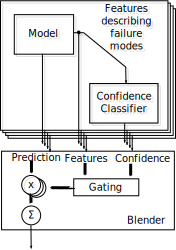
\includegraphics{betterblender}}
\label{fig:ensembling-confidence}
\end{center}
\vskip -0.2in
\end{figure} 

Figure \ref{fig:ensembling-confidence} shows one way to implement such a scheme using a gating function.  The confidence classifiers could either be part of the black box, trained externally from the features, or learnt implicitly as part of the gating function (which would receive only the features).

\subsection{Deep Networks}

The final submission for the small AUC task that is presented in table \ref{table:auc-results} is not in fact the best results that were obtained for this task.  During development of the denoising auto-encoders, an initial auto-encoder was produced that, when trained into a deep network using supervised back-propagation, produced results significantly better than these.  However, due to numerical issues and thread-order non-determinism, these results could not be duplicated nor even closely matched.  There are two possible explanations.  The first is that, in speeding up the code to run at an acceptable speed for the large task, an error was introduced (nearly 2,000 lines of test cases that tested a lot of the invariants in the system).  The second is that these methods are very sensitive and one needs to train many models to fall on a good one\footnote{Of course, one can make one's own luck.  This is why practitioners of deep networks suggest to make them both wide and deep: for each useful generalisation, there is likely to be a neuron somewhere within a wide enough network that will learn it.  Unfortunately, the computational resources were not available to train significantly wider networks than the ones described here.}.

A large amount of effort was also expended to improve the speed of back-propagation, which was were most of the time was spent in training the denoising auto-encoders and deep network models.  The second-order methods indicated in \cite{lecun-98b} were implemented; however they tended to be over-enthusiastic about the learning rate, leading to divergence or oscillation.  Even the simpler methods to generate an overall learning rate failed, and it was necessary to fall back onto manual tuning of parameters.

Perhaps the most important conclusion is that these models are difficult to get right in practise, and would require much experience to use successfully: especially when moved out of the image domain (where most of the successful work has come from) where it is simple to visualise what has been learnt and verify that the models make sense.

\section{Conclusion}

The AUC task proved to be rich and enjoyable, and a significant improvement was obtained on this task, especially on the medium and large datasets.  Models based upon gating of the input models and multiple regressions were successfully used.  Further improvement was achieved by hand-coding features.

The use of unsupervised decompositions to model the joint distribution of the input variables led to some success.  Both a linear SVD decomposition and non-linear denoising auto-encoder decompositions were tried.  The denoising auto-encoder decompositions however did not end up providing good pre-initialisation for deep neural networks, except for on one model which could not be reproduced.  These models appear to be difficult to use well and more experience would have been necessary to use them effectively.

No significant improvements were made on the RMSE task, due to the interplay of a skewed dataset, the presence of noise and the quadratic nature of the RMSE metric.  A less severe metric should be adopted or noise removed from the dataset.  Judging from the leader board on the small task, it is unlikely that any team managed to achieve a significant improvement over the baseline.

An improved model of ensembling was proposed, whereby each model in the ensemble provides not only a prediction of the target function, but a list of features that can be used to determine when the model is likely to be inaccurate.  This model requires further work on the part of the ensemble builders to provide this information, but would allow the ensembling method to have significantly more leverage.

\section*{Acknowledgements} 

Thanks to Phil Brierley for organising and running the challenge.

The \LaTeX\ style file for this report is based upon that for ICML 2009, by P Langley, Terran Lane, Jennifer Dy, Kristian Kersting and Ricardo Silva.


\bibliography{report}
\bibliographystyle{mlapa}

\end{document} 
